% ===================================================================
%  Αρχείο: 14976_tikz.tex (Fragment)
%  Αυτόματη μετατροπή μέσω doc2latex.py & TikZ conversion
% ===================================================================

ΘΕΜΑ 2

Δίνονται τα παρακάτω σχήματα:

\begin{longtable}[]{@{}
  >{\raggedright\arraybackslash}p{(\linewidth - 2\tabcolsep) * \real{0.4999}}
  >{\raggedright\arraybackslash}p{(\linewidth - 2\tabcolsep) * \real{0.5001}}@{}}
\noalign{}

\noalign{}
\endlastfoot

\begin{center}
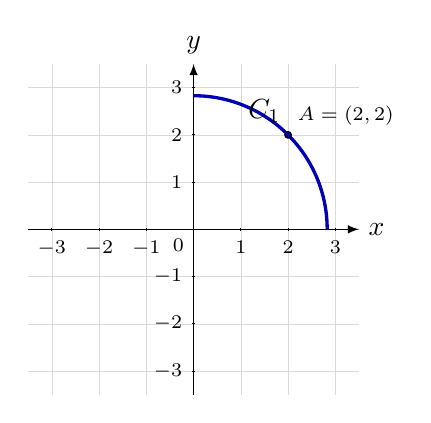
\begin{tikzpicture}[scale=0.6, >=latex]
    \draw[very thin, color=gray!30] (-3.5,-3.5) grid (3.5,3.5);
    \draw[->] (-3.5,0) -- (3.5,0) node[right] {$x$};
    \draw[->] (0,-3.5) -- (0,3.5) node[above] {$y$};
    \foreach \x in {-3,-2,-1,1,2,3}
        \draw (\x,1pt) -- (\x,-1pt) node[below, font=\scriptsize] {$\x$};
    \foreach \y in {-3,-2,-1,1,2,3}
        \draw (1pt,\y) -- (-1pt,\y) node[left, font=\scriptsize] {$\y$};
    \node[below left, font=\scriptsize] at (0,0) {$0$};
    
    \draw[very thick, color=blue!70!black] (2.828,0) arc (0:90:2.828);
    \filldraw[fill=blue!70!black] (2,2) circle (2pt) node[above right, font=\scriptsize] {$A=(2,2)$};
    \node at (1.5,2.5) {$C_1$};
\end{tikzpicture}
\end{center}
 & 
\begin{center}
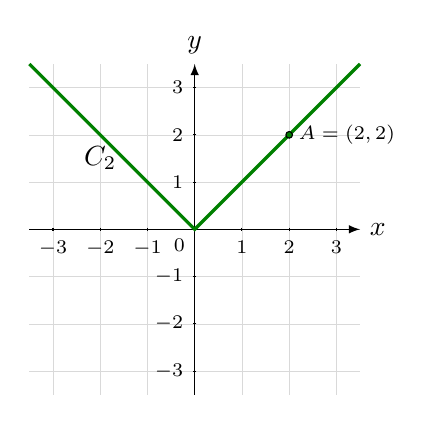
\begin{tikzpicture}[scale=0.6, >=latex]
    \draw[very thin, color=gray!30] (-3.5,-3.5) grid (3.5,3.5);
    \draw[->] (-3.5,0) -- (3.5,0) node[right] {$x$};
    \draw[->] (0,-3.5) -- (0,3.5) node[above] {$y$};
    \foreach \x in {-3,-2,-1,1,2,3}
        \draw (\x,1pt) -- (\x,-1pt) node[below, font=\scriptsize] {$\x$};
    \foreach \y in {-3,-2,-1,1,2,3}
        \draw (1pt,\y) -- (-1pt,\y) node[left, font=\scriptsize] {$\y$};
    \node[below left, font=\scriptsize] at (0,0) {$0$};
    
    \draw[very thick, color=green!50!black] (-3.5,3.5) -- (0,0) -- (3.5,3.5);
    \filldraw[fill=green!50!black] (2,2) circle (2pt) node[right, font=\scriptsize] {$A=(2,2)$};
    \node at (-2,1.5) {$C_2$};
\end{tikzpicture}
\end{center}
 \\

\begin{center}
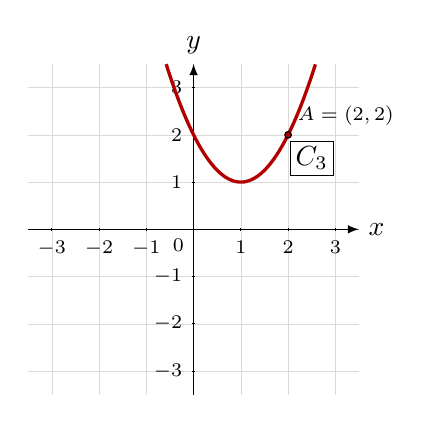
\begin{tikzpicture}[scale=0.6, >=latex]
    \draw[very thin, color=gray!30] (-3.5,-3.5) grid (3.5,3.5);
    \draw[->] (-3.5,0) -- (3.5,0) node[right] {$x$};
    \draw[->] (0,-3.5) -- (0,3.5) node[above] {$y$};
    \foreach \x in {-3,-2,-1,1,2,3}
        \draw (\x,1pt) -- (\x,-1pt) node[below, font=\scriptsize] {$\x$};
    \foreach \y in {-3,-2,-1,1,2,3}
        \draw (1pt,\y) -- (-1pt,\y) node[left, font=\scriptsize] {$\y$};
    \node[below left, font=\scriptsize] at (0,0) {$0$};
    
    \draw[very thick, color=red!70!black, samples=100, domain=-0.58:2.58] plot (\x, {(\x-1)^2 + 1});
    \filldraw[fill=red!70!black] (2,2) circle (2pt) node[above right, font=\scriptsize] {$A=(2,2)$};
    \node at (2.5,1.5) [draw, fill=white, inner sep=2pt] {$C_3$};
\end{tikzpicture}
\end{center}
 & 
\begin{center}
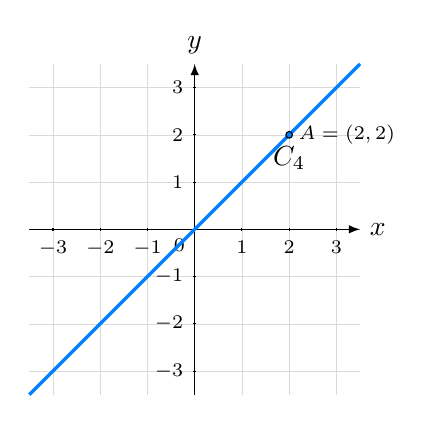
\begin{tikzpicture}[scale=0.6, >=latex]
    \draw[very thin, color=gray!30] (-3.5,-3.5) grid (3.5,3.5);
    \draw[->] (-3.5,0) -- (3.5,0) node[right] {$x$};
    \draw[->] (0,-3.5) -- (0,3.5) node[above] {$y$};
    \foreach \x in {-3,-2,-1,1,2,3}
        \draw (\x,1pt) -- (\x,-1pt) node[below, font=\scriptsize] {$\x$};
    \foreach \y in {-3,-2,-1,1,2,3}
        \draw (1pt,\y) -- (-1pt,\y) node[left, font=\scriptsize] {$\y$};
    \node[below left, font=\scriptsize] at (0,0) {$0$};
    
    \draw[very thick, color=blue!50!cyan] (-3.5,-3.5) -- (3.5,3.5);
    \filldraw[fill=blue!50!cyan] (2,2) circle (2pt) node[right, font=\scriptsize] {$A=(2,2)$};
    \node at (2,1.5) {$C_4$};
\end{tikzpicture}
\end{center}
 \\
\end{longtable}

\begin{alist}
\item Να αιτιολογήσετε ποιες από τις γραφικές παραστάσεις $C_{1},C_{2},C_{3},C_{4}$ αναπαριστούν άρτιες ή περιττές συναρτήσεις, ποιες όχι και γιατί. Δίνεται ότι τουλάχιστον μία είναι άρτια και τουλάχιστον μία είναι περιττή.

\monades{12}

\item Για τις συναρτήσεις $C_{2},C_{4}$ να βρείτε την τεταγμένη του σημείου τους $Β( - 2,k),$ αιτιολογώντας την τιμή που βρήκατε από την ιδιότητα συμμετρίας καθεμίας συνάρτησης.

\monades{13}
\end{alist}
